\chapter{Исследовательская часть}

\section{Технические характеристики}

Технические характеристики устройства, на котором выполнялись замеры по времени, представлены далее.

\begin{itemize}
	\item Процессор: AMD Ryzen 5 5500U\,--\,2.10 GHz;
	\item Оперативная память: 16 ГБайт;
	\item Операционная система: Windows 10 Pro 64-разрядная система версии 22H2~\cite{windows}.
\end{itemize}

При замерах времени ноутбук был включен в сеть электропитания и был нагружен только системными приложениями.

\section{Демонстрация работы программы}

На рисунке \ref{img:demonstration} представлена демонстрация работы разработанного ПО, а именно показаны результаты работы алгоритмов поиска расстояний Левенштейна и Дамерау\,--\,Левенштейна на примере двух строк \textit{<<секста>>} и \textit{<<септима>>}.  
\clearpage
\begin{figure}[h]
	\centering
	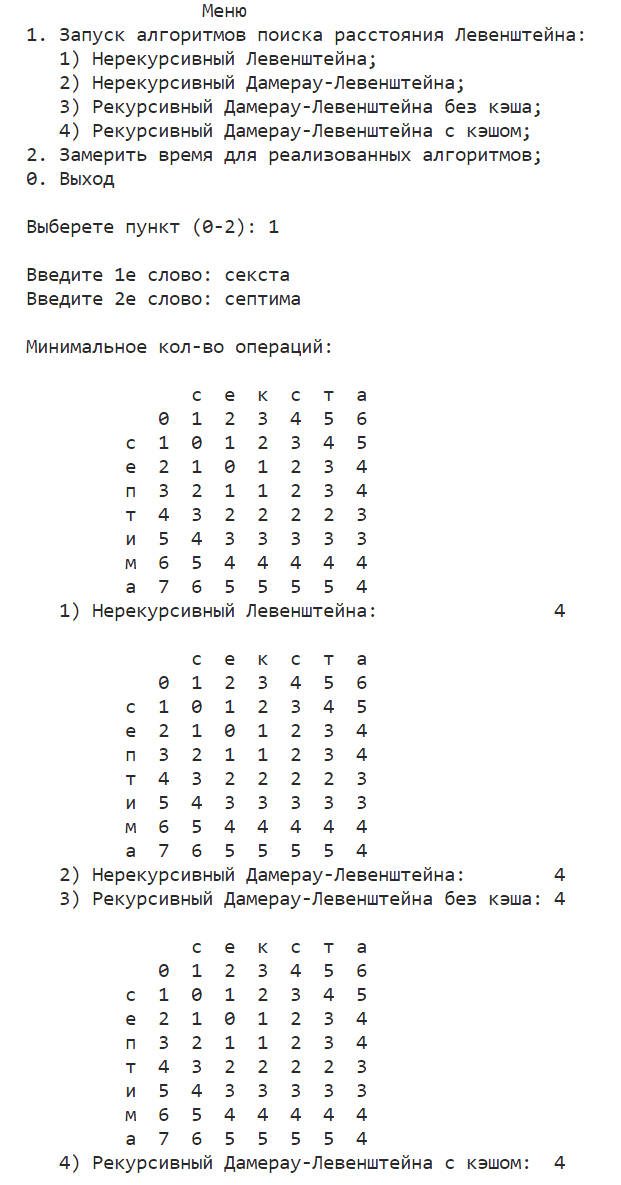
\includegraphics[height=0.7\textheight]{img/prog_work.png}
	\caption{Демонстрация работы программы}
	\label{img:demonstration}
\end{figure}

\clearpage

\section{Временные характеристики}

Все реализованный алгоритмы сравнивались на случайно сгенерированных строках длиной:
\begin{itemize}
	\item 0--10 с шагом 1 для всех алгоритмов;
	\item 10--100 с шагом 10 для нерекурсивных и рекурсивного с кешированием 
\end{itemize}
Поскольку замеры по времени имеют некоторую погрешность, для каждой строки и каждой реализации алгоритма замеры производились 1000 раз, а затем вычислялось среднее арифметическое значение.

На рисунке \ref{plt:time_02} представлен график, иллюстрирующий зависимость времени работы от длины строк для матричных реализаций алгоритмов поиска расстояний Левенштейна и Дамерау\,--\,Левенштейна. Время их работы растет соизмеримо, но алгоритм поиска расстояния Дамерау\,--\,Левенштейна работает дольше, так как в нем присутствует дополнительная проверка для обмена соседних символов.
\begin{figure}[h]
	\centering
	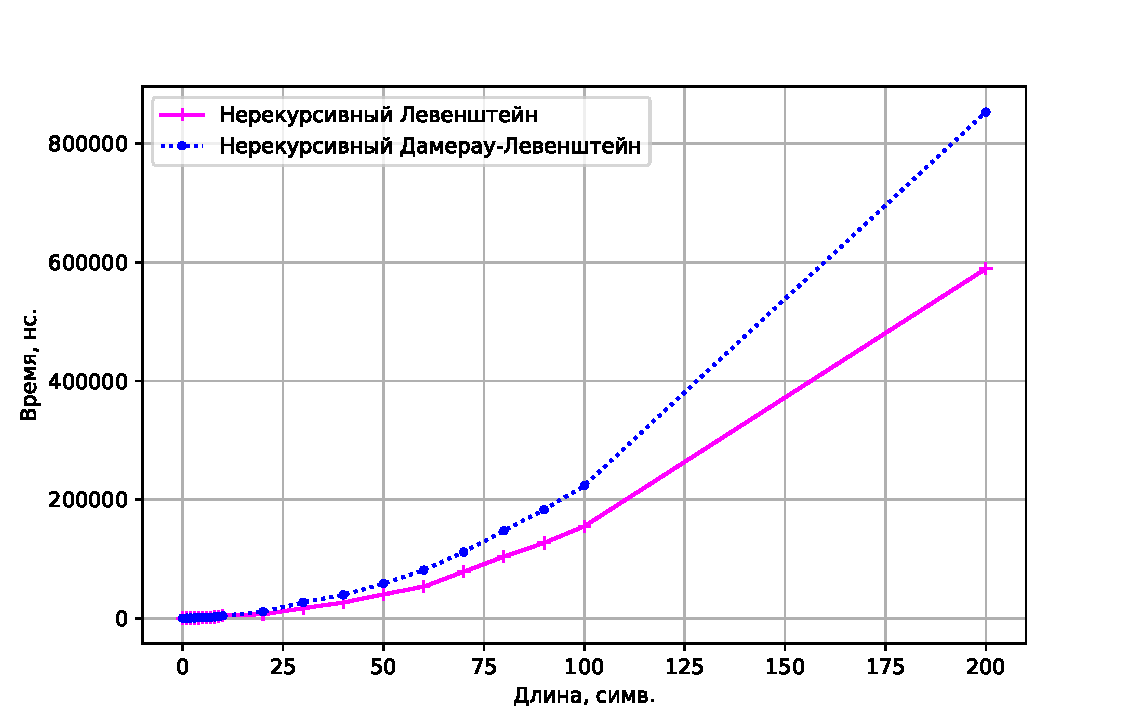
\includegraphics[height=0.4\textheight, page=1]{img/figures.pdf}
	\caption{Сравнение по времени матричных реализаций алгоритмов поиска расстояний Левенштейна и Дамерау\,--\,Левенштейна}
	\label{plt:time_01}
\end{figure}

На рисунке \ref{plt:time_02} представлен график, иллюстрирующий зависимость времени работы от длины строк для рекурсивных реализаций алгоритмов поиска расстояния Дамерау\,--\,Левенштейна с кешем и без.

\begin{figure}[h]
	\centering
	\includegraphics[height=0.5\textheight, page=2]{img/figures.pdf}
	\caption{Сравнение по времени рекурсивных реализаций алгоритмов поиска расстояния Дамерау\,--\,Левенштейна с кешем и без}
	\label{plt:time_02}
\end{figure}

На рисунке \ref{plt:time_03} представлен график, иллюстрирующий зависимость времени работы от длины строк для матричных реализаций. На графике видно, что матричные реализации работают значительно быстрее рекурсивной реализации с кешированием. 

\begin{figure}[h]
	\centering
	\includegraphics[height=0.5\textheight, page=3]{img/figures.pdf}
	\caption{Сравнение по времени матричных реализаций алгоритмов поиска расстояния Левенштейна и Дамерау\,--\,Левенштейна и рекурсивной реализации с кешем поиска расстояния Дамерау\,--\,Левенштейна}
	\label{plt:time_03}
\end{figure}

\section{Характеристики по памяти}

Введем следующие обозначения:
\begin{itemize}
	\item$n$~--- длина строки $S_{1}$;
	\item$m$~--- длина строки $S_{2}$;
	\item$size()$~--- функция вычисляющая размер в байтах;
	\item $char$~--- тип, используемый для хранения символа строки;
	\item $int$~--- целочисленный тип;
\end{itemize}

Использование памяти при \textbf{итеративной реализации} алгоритма поиска расстояния Левенштейна теоретически равно:
\begin{equation}
	\label{eq:lev_mtr_memory}
	\begin{aligned}
		M_{iter} = (m + 1) \cdot (n + 1) \cdot size(int) + (n + m) \cdot size(char) + \\ + 5 \cdot size(int) + size(int **) + (n + 1) \cdot size(int *),
	\end{aligned}
\end{equation}
где: 
\begin{itemize}
	\item $(n + 1) \cdot (m + 1) \cdot size(int)$~--- хранение матрицы;
	\item $(n + m) \cdot size(char)$~--- хранение двух строк;
	\item $2 \cdot size(int)$~--- хранение размеров строк;
	\item $3 \cdot size(int)$~--- дополнительные переменные;
	\item $size(int**) + (n + 1) \cdot size(int *)$~--- указатель на матрицу;
\end{itemize}

Использование памяти при \textbf{итеративной реализации} алгоритма поиска расстояния Дамерау\,--\,Левенштейна идентично формуле \ref{eq:lev_mtr_memory}.

Рассчитаем затраты по памяти для \textbf{рекурсивного} алгоритма поиска расстояния Дамерау\,--\,Левенштейна\textit{ (для каждого вызова)}:
\begin{equation}
	\label{}
	\begin{aligned}
		M_{call} = (m + n) \cdot size(char) + 4 \cdot size(int) + 8 байт
	\end{aligned}
\end{equation}
где: 
\begin{itemize}
	\item $(n + m) \cdot size(char)$~--- хранение двух строк;
	\item $2 \cdot size(int)$~--- хранение размеров строк;
	\item $2 \cdot size(int)$~--- дополнительные переменные;
	\item 8 байт~--- адрес возврата.
\end{itemize}

Макисмальная глубина стека вызовов при рекурсивной реализации равна сумме длин входящий строк, поэтому макисмальный расход памяти равен:
\begin{equation}
	\label{}
	\begin{aligned}
		M_{rec} = (n + m) \cdot M_{call}
	\end{aligned}
\end{equation}
где: 
\begin{itemize}
    \item $n + m$~--- максимальная глубина стека;
	\item $M_{call}$~--- затраты по памяти для одного рекурсивного вызова.
\end{itemize}

Для рекурсивного алгоритма поиска расстояния Дамерау\,--\,Левенштейна с использованием кеша необходимо подсчитать размер самого кеша:
\begin{equation}
	\label{}
	\begin{aligned}
		M_{cash} = (m + 1) \cdot (n + 1) \cdot size(int) + size(int **) + (n + 1) \cdot size(int *)
	\end{aligned}
\end{equation}
где: 
\begin{itemize}
    \item $(m + 1) \cdot (n + 1)$~--- количество элементов в кеше;
	\item $size(int **) + (n + 1) \cdot size(int *)$~--- хранение указателей.
\end{itemize}

Затраты по памяти для рекурсивного алгоритма поиска расстояния Дамерау\,--\,Левенштейна с учетом кеша: 
\begin{equation}
	\label{}
	\begin{aligned}
		M_{recCash} = M_{rec} + M_{cash}
	\end{aligned}
\end{equation}

\section{Вывод}
TODO
Алгоритм нахождения расстояния Дамерау\,--\,Левенштейна по времени выполнения незначительно отличается от алгоритма нахождения расстояния Левенштейна.

Рекурсивные реализации поиска расстояния Дамерау\,--\,Левенштейна работают на порядок дольше матричной реализации.

По расходу памяти матричный алгоритм проигрывает рекурсивному: макисмальный размер используемой памяти у матричного алгоритма растет как \textit{произведение} длиин строк, а то время как у рекурсивного - как \textit{сумма} длин строк.